\documentclass[14pt]{beamer}
\usetheme{Montpellier}
\usecolortheme{beaver}

\title{Variational Inference: The Basics}
\date{}
\author[Schulz and Aziz]{Philip Schulz and Wilker Aziz}

\usepackage{amsmath, amssymb, ../../vimacros, hyperref, enumerate}
\usepackage[round]{natbib}

\hypersetup{breaklinks=true, colorlinks=true, linkcolor=blue, citecolor=blue, urlcolor=blue}

\usepackage{tikz}
\usetikzlibrary{bayesnet}

\begin{document}

\frame{\titlepage}

\section{Generative Models}

\begin{frame}{Joint Distribution}
Let $ X $ and $ Z $ be random variables. A generative model is any model that defines a joint distribution
over these variables. 
\pause
\begin{block}{2 Examples of Generative Models}
\begin{itemize}
\item $ p(x,z) = p(x) p(z|x) $
\item $ p(x,z) = p(z) p(x|z) $
\end{itemize}
\end{block}
\end{frame}

\begin{frame}{Likelihood and prior}
From here on, $ x $ is our observed data. On the other hand, $ z $ is an unobserved outcome. 
\begin{itemize}
\item $ p(x|z) $ is the \textbf{likelihood}
\item $ p(z) $ is the \textbf{prior} over $ Z $
\end{itemize} 
Notice: the prior may depend on a non-random quantity $ \alpha $ (write $ p(z|\alpha) $). In that case, we 
call $ \alpha $ a hyperparameter.
\end{frame}

\begin{frame}{Bayes' rule}
Bayes rule asserts that we can \textit{invert} a conditional probability distribution.
\begin{equation}
p(z|x) = \frac{p(x|z)p(z)}{p(x)}
\end{equation}
\end{frame}

\begin{frame}{Bayes' rule}
Bayes rule asserts that we can \textit{invert} a conditional probability distribution.
\begin{equation}
p(z|x) = \frac{\overbrace{p(x|z)}^{\text{likelihood}}\overbrace{p(z)}^{prior}}{p(x)}
\end{equation}
\end{frame}

\begin{frame}{Bayes' rule}
Bayes rule asserts that we can \textit{invert} a conditional probability distribution.
\begin{equation}
\underbrace{p(z|x)}_{\text{posterior}} = \frac{\overbrace{p(x|z)}^{\text{likelihood}}\overbrace{p(z)}^{prior}}{p(x)}
\end{equation}
\end{frame}

\begin{frame}{Bayes' rule}
Bayes rule asserts that we can \textit{invert} a conditional probability distribution.
\begin{equation}
\underbrace{p(z|x)}_{\text{posterior}} = \frac{\overbrace{p(x|z)}^{\text{likelihood}}\overbrace{p(z)}^{\text{prior}}}{\underbrace{p(x)}_{\text{\alert{marginal likelihood/evidence}}}}
\end{equation}
\end{frame}

\begin{frame}{The Basic Problem}
We want to compute the posterior over latent variables $ p(z|x) $. This involves computing the marginal likelihood
$$ p(x) = \intl{ p(x,z) }{z} $$
which is often \textbf{intractable}. This problem motivates the use of \textbf{approximate inference} techniques.
\end{frame}

\begin{frame}{Bayesian Inference}
Model parameters $ \theta $ are also random. The generative model becomes
\begin{itemize}
\item $ p(x,\theta) $ for fully observed data (supervised learning)
\item $ p(x,z,\theta) $ for observed and latent data \\ (unsupervised learning)
\end{itemize}
\end{frame}

\begin{frame}{Bayesian Inference}
The evidence becomes even harder to compute because $ \theta $ is often high-dimensional
(just think of neural nets!).
\begin{itemize}
\item $ p(x) = \intl{ p(x, \theta)}{\theta} $ (supervised learning)
\item $ p(x) = \intl{ \int{ p(x, z, \theta)} {z}}{\theta} $ (unsupervised learning)
\end{itemize}
\pause
Again, approximate inference is needed.
\end{frame}

\section{Examples}

\begin{frame}{Factorial HMMs}
FHMMs have several Markov chains over latent variables.
\begin{figure}
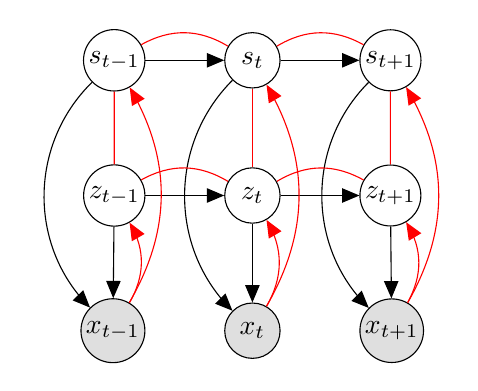
\begin{tikzpicture}
\node[obs] (xt) {$ x_{t} $};
\node[obs, left=of xt] (xt-1) {$ x_{t-1} $};
\node[obs, right=of xt] (xt+1) {$ x_{t+1} $};

\node[latent, above= of xt] (zt) {$ z_{t} $};
\node[latent, left= of zt] (zt-1) {$ z_{t-1} $};
\node[latent, right= of zt] (zt+1) {$ z_{t+1} $};

\node[latent, above= of zt] (st) {$ s_{t} $};
\node[latent, left= of st] (st-1) {$ s_{t-1} $};
\node[latent, right= of st] (st+1) {$ s_{t+1} $};

\edge {zt} {xt, zt+1};
\edge {zt-1} {xt-1, zt};
\edge {zt+1} {xt+1};

\edge {st-1} {st};
\edge {st} {st+1};

% bend edges don't work in bayesnet and need to be created by hand.
\path (st-1) edge[bend right=45, ->] (xt-1);
\path (st) edge[bend right=45, ->] (xt);
\path (st+1) edge[bend right=45, ->] (xt+1);

\pause
% inference edges
\path (xt-1) edge[->, color=red, bend right=30] (zt-1);
\path (xt) edge[->, color=red, bend right=30] (zt);
\path (xt+1) edge[->, color=red, bend right=30] (zt+1);

\path (xt-1) edge[->, color=red, bend right=30] (st-1);
\path (xt) edge[->, color=red, bend right=30] (st);
\path (xt+1) edge[->, color=red, bend right=30] (st+1);

\pause
\edge[-, color=red]{st-1}{zt-1};
\edge[-, color=red]{st}{zt};
\edge[-, color=red]{st+1}{zt+1};

\pause
\path (st-1) edge[-, color=red, bend left=30] (st);
\path (st) edge[-, color=red, bend left=30] (st+1);
\path (zt-1) edge[-, color=red, bend left=30] (zt);
\path (zt) edge[-, color=red, bend left=30] (zt+1);
\end{tikzpicture}
\end{figure}
\end{frame}

\begin{frame}{Factorial HMMs}
Inference network for FHHMs.
\begin{figure}
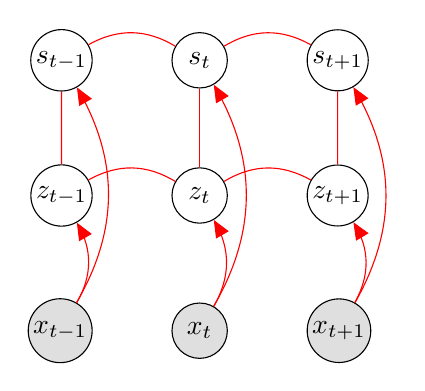
\begin{tikzpicture}
\node[obs] (xt) {$ x_{t} $};
\node[obs, left=of xt] (xt-1) {$ x_{t-1} $};
\node[obs, right=of xt] (xt+1) {$ x_{t+1} $};

\node[latent, above= of xt] (zt) {$ z_{t} $};
\node[latent, left= of zt] (zt-1) {$ z_{t-1} $};
\node[latent, right= of zt] (zt+1) {$ z_{t+1} $};

\node[latent, above= of zt] (st) {$ s_{t} $};
\node[latent, left= of st] (st-1) {$ s_{t-1} $};
\node[latent, right= of st] (st+1) {$ s_{t+1} $};

% inference edges
\path (xt-1) edge[->, color=red, bend right=30] (zt-1);
\path (xt) edge[->, color=red, bend right=30] (zt);
\path (xt+1) edge[->, color=red, bend right=30] (zt+1);

\path (xt-1) edge[->, color=red, bend right=30] (st-1);
\path (xt) edge[->, color=red, bend right=30] (st);
\path (xt+1) edge[->, color=red, bend right=30] (st+1);

\edge[-, color=red]{st-1}{zt-1};
\edge[-, color=red]{st}{zt};
\edge[-, color=red]{st+1}{zt+1};

\path (st-1) edge[-, color=red, bend left=30] (st);
\path (st) edge[-, color=red, bend left=30] (st+1);
\path (zt-1) edge[-, color=red, bend left=30] (zt);
\path (zt) edge[-, color=red, bend left=30] (zt+1);
\end{tikzpicture}
\end{figure}
\end{frame}

\begin{frame}{Factorial HMMs}
FHMMs have several Markov chains over latent variables.
\begin{itemize}
\item $ M $ Markov chains over latent variables.
\item $ L $ outcomes per latent variable.
\item Sequence of length $ T $.
\item Complexity of inference: $ \mathcal{O}(L^{2M}T) $.
\end{itemize}
\pause
\begin{alertblock}{Intractable}
Exponential dependency on the number of hidden Markov chains.
\end{alertblock}
\end{frame}

\begin{frame}{Latent Dirichlet Allocation}
An admixture model that changes its mixture weights per document. We assume that the mixture components
are fixed.
\begin{figure}
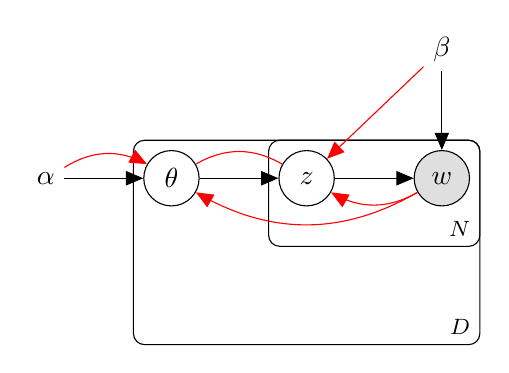
\begin{tikzpicture}
\node[obs] (w) {$ w $};
\node[latent, left= of w] (z) {$ z $};
\node[latent, left= of z] (theta) {$ \theta $};
\node[left= of theta] (alpha) {$ \alpha $};
\node[above= of w] (beta) {$ \beta $};
\node[below= of z] (fake) {}; % needed to fit the document plate

\plate {tokens} {(w)(z)} {$ N $};
\plate {document} {(w)(z)(theta)(fake)} {$ D $};

\edge {alpha} {theta};
\edge {theta} {z};
\edge {z} {w};
\edge {beta} {w};

\pause
% inference edges
\path (w) edge[->,bend left=30,color=red] (z);
\path (w) edge[->,bend left=30,color=red] (theta);
\edge[color=red] {beta} {z};
\pause
\path (z) edge[-,bend right=30,color=red] (theta);
\path (alpha) edge[->, bend left=30, color=red] (theta);
\end{tikzpicture}
\end{figure}
\end{frame}

\begin{frame}{Latent Dirichlet Allocation}
Inference network for LDA.
\begin{figure}
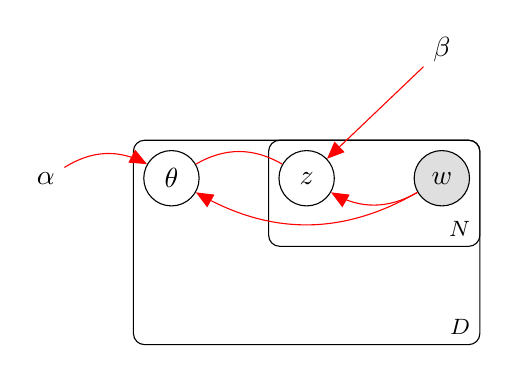
\begin{tikzpicture}
\node[obs] (w) {$ w $};
\node[latent, left= of w] (z) {$ z $};
\node[latent, left= of z] (theta) {$ \theta $};
\node[left= of theta] (alpha) {$ \alpha $};
\node[above= of w] (beta) {$ \beta $};
\node[below= of z] (fake) {}; % needed to fit the document plate

\plate {tokens} {(w)(z)} {$ N $};
\plate {document} {(w)(z)(theta)(fake)} {$ D $};

% inference edges
\path (w) edge[->,bend left=30,color=red] (z);
\path (w) edge[->,bend left=30,color=red] (theta);
\path (z) edge[-,bend right=30,color=red] (theta);
\path (alpha) edge[->, bend left=30, color=red] (theta);
\edge[color=red] {beta} {z};
\end{tikzpicture}
\end{figure}
\end{frame}

\begin{frame}{Latent Dirichlet Allocation}
An admixture model that changes its mixture weights per document. Here we assume that the mixture components
are fixed.
\begin{itemize}
\item $ D $ documents.
\item $ N $ tokens and latent variables per document.
\item $ L $ outcomes per latent variable.
\item Complexity of inference: $ \mathcal{O}(L^{DN}) $.
\end{itemize}
\end{frame}

\section{Variational Inference}

\begin{frame}{The Goal}
Assume $ p(z|x) $ is intractable.
\pause
\begin{block}{Idea}
Let's approximate it by an auxiliary distribution $ q(z) $ that is tractable!
\end{block}
\pause
\begin{block}{Requirement}
Choose $ q(z) $ as close as possible to $ p(z|x) $ to obtain a faithful approximation.
\end{block}
\pause
\begin{block}{Implementation}
Minimize $ \KL{q(z)}{p(z|x)} $.
\end{block}
\end{frame}

\begin{frame}{Recap KL divergence}
The Kullback-Leibler divergence (or relative entropy) measures the divergence of a distribution $ q $ from 
a distribution $ q $. 
\begin{itemize}
\item $ \KL{q(z)}{p(z|x)} = \intl{ q(z) \loga{\frac{q(z)}{p(z|x)}}}{z} $ (continuous)
\item $ \KL{q(z)}{p(z|x)} = \sum_{z} q(z) \loga{\frac{q(z)}{p(z|x)}} $ (discrete)
\item $ \KL{q(z)}{p(z|x)} = \E[q(z)]{\loga{\frac{q(z)}{p(z|x)}}} $ (both)
\end{itemize}
\end{frame}

\begin{frame}{Recap KL divergence}
\begin{block}{Properties}
\begin{itemize}
\item $ \KL{q(z)}{p(z|x)} \geq 0 $ with \\ equality iff $ q(z) = p(z|x) $.
\pause
\item $ \KL{q(z)}{p(z|x)} = \infty $ \\ if $ \exists z $ s.t. $ p(z|x) = 0 $ and $ q(z) > 0 $.
\pause
\item In general $ \KL{q(z)}{p(z|x)} \not = \KL{p(z|x)}{q(z)} $.
\pause
\item $ -\KL{q(z)}{p(z|x)} \leq 0 $.
\end{itemize}
\end{block}
\end{frame}

\subsection{Deriving VI with Jensen's Inequality}

\begin{frame}{VI derivation I}
\begin{small}
\begin{align*}
\log p(x) &= \loga{\intl{p(x,z)}{z}} \\
&= \loga{\intl{\alert{q(z)}\frac{p(x,z)}{\alert{q(z)}}}{z}} \\
&\geq \intl{ \alert{q(z)} \loga{\frac{p(x,z)}{\alert{q(z)}}}} {z} \\
& = \intl{ \alert{q(z)} \loga{\frac{p(z|x)p(x)}{\alert{q(z)}}}} {z} \\
&= \intl{ \alert{q(z)} \loga{\frac{p(z|x)}{\alert{q(z)}}}} {z} + \log p(x)
\end{align*}
\end{small}
\end{frame}

\begin{frame}{VI derivation I}
\begin{small}
\begin{align*}
\intl{ q(z) \loga{\frac{p(z|x)}{q(z)}}}{z} + \loga{p(x)} \\
= -\KL{q(z)}{p(z|x)} + \loga{p(x)}
\end{align*}
\end{small}
We have derived a lower bound on the log-evidence whose gap is exactly $ \KL{q(z)}{p(z|x)} $.
\end{frame}

\subsection{Deriving VI from KL Divergence}

\begin{frame}{VI derivation II}
Recall that we want to find $ q(z) $ such that $ \KL{q(z)}{p(z|x)} $ is small.
\pause
\begin{block}{Formal Objective}
\begin{equation*}
\underset{q(z)}{\min} \KL{q(z)}{p(z|x)} = \underset{q(z)}{\max} -\KL{q(z)}{p(z|x)}
\end{equation*}
\end{block}
\end{frame}

\begin{frame}{VI derivation II}
\begin{small}
\begin{align*}
&\underset{q(z)}{\max} -\KL{q(z)}{p(z|x)} \\ 
&= \underset{q(z)}{\max} \intl{ q(z) \loga{\frac{p(z|x)}{q(z)}}}{z} \\
&= \underset{q(z)}{\max} \intl{ q(z) \loga{\frac{p(z,x)}{p(x)q(z)}}} {z} \\
&= \underset{q(z)}{\max} \intl{ q(z) \loga{p(z,x)}} {z} - \intl{ q(z) \loga{q(z)}} {z} 
- \overbrace{\log(p(x))}^{constant} \\
&= \underset{q(z)}{\max}~\E[q(z)]{\loga{p(x,z)}} + \Ent{q(z)}
\end{align*}
\end{small}
\end{frame}

\begin{frame}
As before, we have derived a lower bound on the log-evidence. This \textbf{evidence lower bound}
or \textbf{ELBO} is our optimisation objective.
\begin{block}{ELBO}
\begin{equation*}
\underset{q(z)}{\max}~\E[q(z)]{\loga{p(x,z)}} + \Ent{q(z)}
\end{equation*}
\end{block}
\end{frame}

\subsection{Relationship to EM}

\begin{frame}{Performing VI}
VI in its basic form can be performed via coordinate ascent. This can be done as a 2-step procedure.
\begin{enumerate}
\pause
\item Compute the expected log-density $ \E[q(z)]{\loga{p(x,z)}} $.
\pause
\item Maximize with respect to $ q(z) $ and while trying to keep $ q(z) $ as broad as possible (through entropy
regularisation):
\begin{equation}
\underset{q(z)}{\max}~\E[q(z)]{\loga{p(x,z)}} + \Ent{q(z)}
\end{equation}
\end{enumerate}
\end{frame}

\begin{frame}{What if $ q(z) = p(z|x) $?}
If $ q(z) = p(z|x) $ then $ \KL{q(z)}{p(z|x)} = 0 $ and thus we are directly optimising the log-evidence.
\begin{enumerate}
\item Compute the expected log-density $ \E[p(z|x)]{\loga{p(x,z)}} $.
\item Maximize with respect to $ p(z|x) $ and while trying to keep $ p(z|x) $ as broad as possible (through entropy
regularisation):
\begin{equation}
\underset{p(z|x)}{\max}~\E[p(z|x)]{\loga{p(x,z)}} + \Ent{p(z|x)}
\end{equation}
\end{enumerate}
\end{frame}

\begin{frame}{What if $ q(z) = p(z|x) $?}
If $ q(z) = p(z|x) $ then $ \KL{q(z)}{p(z|x)} = 0 $ and thus we are directly optimising the log-evidence.
\begin{itemize}
\item[\alert{E-step}] $ \E[p(z|x)]{\loga{p(x,z)}} $.
\item[\alert{M-step}] Maximize with respect to $ p(z|x) $ and while trying to keep $ p(z|x) $ as broad as possible 
(through entropy regularisation):
\begin{equation}
\underset{p(z|x)}{\max}~\E[p(z|x)]{\loga{p(x,z)}} + \Ent{p(z|x)}
\end{equation}
\end{itemize}
\end{frame}

\begin{frame}{Relationship to EM}
\begin{itemize}
\item Variational Inference where $ q(z) = p(z|x) $ is EM!
\item The E-step does not change except
that we are using $ q(z) $ to compute the expected density.
\begin{equation*}
\E[q(z)]{\loga{p(x,z)}} \not = \E[p(z|x)]{\loga{p(x,z)}}
\end{equation*}
\item The M-step depends on what family we chose for $ q(z) $.
\pause
\alert{This may be a different family than $ p(z|x) $!}
\end{itemize}
\end{frame}

\subsection{Mean Field Inference}

\begin{frame}{Designing a tractable approximation}
\begin{itemize}
\item Recall: The approximation $ q(z) $ needs to be tractable.
\item Common solution: make \textbf{all} latent variables independent under $ q(z) $.
\pause
\item Formal assumption: $ q(z) = \prod_{i=1}^{N}q(z_{i}) $
\end{itemize}
\pause
This approximation strategy is commonly known as \textbf{mean field} approximation.
\end{frame}

\begin{frame}{Original FHHM Inference} 
\begin{figure}
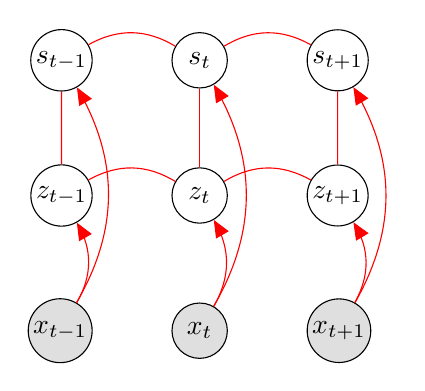
\begin{tikzpicture}
\node[obs] (xt) {$ x_{t} $};
\node[obs, left=of xt] (xt-1) {$ x_{t-1} $};
\node[obs, right=of xt] (xt+1) {$ x_{t+1} $};

\node[latent, above= of xt] (zt) {$ z_{t} $};
\node[latent, left= of zt] (zt-1) {$ z_{t-1} $};
\node[latent, right= of zt] (zt+1) {$ z_{t+1} $};

\node[latent, above= of zt] (st) {$ s_{t} $};
\node[latent, left= of st] (st-1) {$ s_{t-1} $};
\node[latent, right= of st] (st+1) {$ s_{t+1} $};

% inference edges
\path (xt-1) edge[->, color=red, bend right=30] (zt-1);
\path (xt) edge[->, color=red, bend right=30] (zt);
\path (xt+1) edge[->, color=red, bend right=30] (zt+1);

\path (xt-1) edge[->, color=red, bend right=30] (st-1);
\path (xt) edge[->, color=red, bend right=30] (st);
\path (xt+1) edge[->, color=red, bend right=30] (st+1);

\edge[-, color=red]{st-1}{zt-1};
\edge[-, color=red]{st}{zt};
\edge[-, color=red]{st+1}{zt+1};

\path (st-1) edge[-, color=red, bend left=30] (st);
\path (st) edge[-, color=red, bend left=30] (st+1);
\path (zt-1) edge[-, color=red, bend left=30] (zt);
\path (zt) edge[-, color=red, bend left=30] (zt+1);
\end{tikzpicture}
\end{figure}
\center{Exact posterior $ p(s,z|x) $}
\end{frame}

\begin{frame}{Mean field FHHM Inference}
\begin{figure}
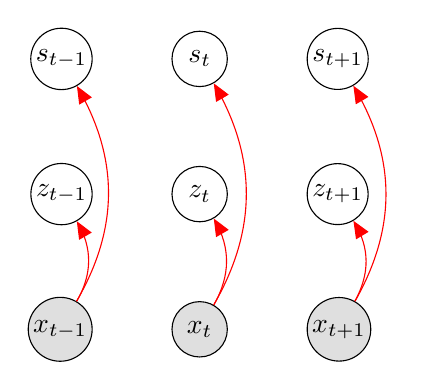
\begin{tikzpicture}
\node[obs] (xt) {$ x_{t} $};
\node[obs, left=of xt] (xt-1) {$ x_{t-1} $};
\node[obs, right=of xt] (xt+1) {$ x_{t+1} $};

\node[latent, above= of xt] (zt) {$ z_{t} $};
\node[latent, left= of zt] (zt-1) {$ z_{t-1} $};
\node[latent, right= of zt] (zt+1) {$ z_{t+1} $};

\node[latent, above= of zt] (st) {$ s_{t} $};
\node[latent, left= of st] (st-1) {$ s_{t-1} $};
\node[latent, right= of st] (st+1) {$ s_{t+1} $};

% inference edges
\path (xt-1) edge[->, color=red, bend right=30] (zt-1);
\path (xt) edge[->, color=red, bend right=30] (zt);
\path (xt+1) edge[->, color=red, bend right=30] (zt+1);

\path (xt-1) edge[->, color=red, bend right=30] (st-1);
\path (xt) edge[->, color=red, bend right=30] (st);
\path (xt+1) edge[->, color=red, bend right=30] (st+1);
\end{tikzpicture}
\end{figure}
\center{Approximate posterior $ q(s,z) = \prod_{t=1}^{T}q(s_{t})q(z_{t})$}
\end{frame}

\begin{frame}{Original LDA Inference}
\begin{figure}
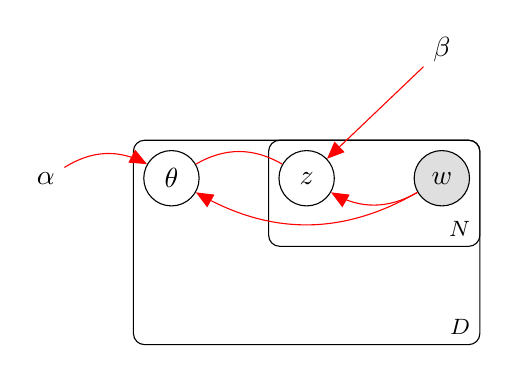
\begin{tikzpicture}
\node[obs] (w) {$ w $};
\node[latent, left= of w] (z) {$ z $};
\node[latent, left= of z] (theta) {$ \theta $};
\node[left= of theta] (alpha) {$ \alpha $};
\node[above= of w] (beta) {$ \beta $};
\node[below= of z] (fake) {}; % needed to fit the document plate

\plate {tokens} {(w)(z)} {$ N $};
\plate {document} {(w)(z)(theta)(fake)} {$ D $};

% inference edges
\path (w) edge[->,bend left=30,color=red] (z);
\path (w) edge[->,bend left=30,color=red] (theta);
\path (z) edge[-,bend right=30,color=red] (theta);
\path (alpha) edge[->, bend left=30, color=red] (theta);
\edge[color=red] {beta} {z};
\end{tikzpicture}
\end{figure}
\center{Exact posterior $ p(z,\theta|w,\alpha, \beta) $}
\end{frame}

\begin{frame}{Mean field LDA Inference}
\begin{figure}
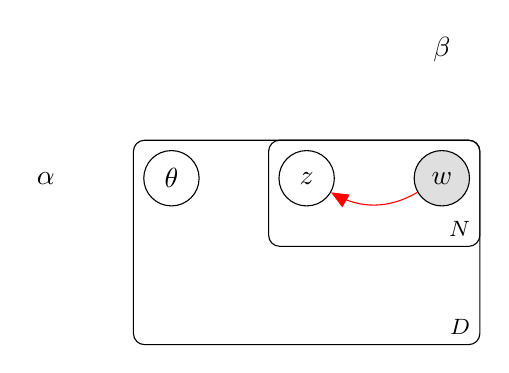
\begin{tikzpicture}
\node[obs] (w) {$ w $};
\node[latent, left= of w] (z) {$ z $};
\node[latent, left= of z] (theta) {$ \theta $};
\node[left= of theta] (alpha) {$ \alpha $};
\node[above= of w] (beta) {$ \beta $};
\node[below= of z] (fake) {}; % needed to fit the document plate

\plate {tokens} {(w)(z)} {$ N $};
\plate {document} {(w)(z)(theta)(fake)} {$ D $};

% inference edges
\path (w) edge[->,bend left=30,color=red] (z);
\end{tikzpicture}
\end{figure}
\center{Approximate posterior $ q(z,\theta|w,\alpha, \beta) = \prod_{d=1}^{D}q(\theta_{d})\prod_{i=1}^{N}q(z_i|w) $}
\end{frame}

\section{Summary}

\begin{frame}{Summary}
\begin{itemize}
\item Posterior inference is often \textbf{intractable} because the marginal likelihood (or \textbf{evidence}) 
$ p(x) $ cannot be computed efficiently.
\item Variational inference approximates the posterior $ p(z|x) $ with a simpler distribution $ q(z) $.
\item The variational objective is the \textbf{evidence lower bound (ELBO)}:
\begin{equation}
\E[q(z)]{\loga{p(x,z)}} + \Ent{q(z)}
\end{equation}
\end{itemize}
\end{frame}

\begin{frame}{Summary}
\begin{itemize}
\item The \textbf{ELBO} is a lower bound on the log-evidence.
\item When $ q(z) = p(z|x) $ we recover EM.
\item A common approximation is the \textbf{mean field} approximation which assumes that all latent variables
are independent:
\begin{equation*}
q(z) = \prod_{i=1}^{N} q(z_{i})
\end{equation*}
\end{itemize}
\end{frame}

\section{Literature}

\nocite{BleiEtAl:2016}
\nocite{NealHinton:1998}
\nocite{GhahramaniJordan:1996}
\nocite{BleiEtAl:2003}

\begin{frame}[allowframebreaks]{Literature}
\bibliographystyle{plainnat}
\small
\bibliography{../../VI}
\end{frame}

\end{document}
